\documentclass[11pt,a4paper]{article}
\usepackage[margin=2.5cm]{geometry}
\usepackage{amsmath,amssymb}
\usepackage{graphicx}
\usepackage{booktabs}
\usepackage{hyperref}
\usepackage[T1]{fontenc}
\usepackage{lmodern}
\usepackage{xcolor}
\usepackage{pifont}
\newcommand{\cmark}{\ding{51}}
\newcommand{\xmark}{\ding{55}}
\usepackage{enumitem}
\usepackage{listings}
\usepackage{float}

\hypersetup{colorlinks=true,linkcolor=blue!60!black,citecolor=blue!60!black,urlcolor=blue!60!black}

\lstset{
  language=Python,
  basicstyle=\ttfamily\small,
  keywordstyle=\color{blue!70!black}\bfseries,
  commentstyle=\color{green!50!black}\itshape,
  stringstyle=\color{red!60!black},
  showstringspaces=false,
  frame=single,
  framerule=0.4pt,
  rulecolor=\color{gray!50},
  backgroundcolor=\color{gray!5},
  breaklines=true,
  numbers=left,
  numberstyle=\tiny\color{gray},
  xleftmargin=2em,
}

\title{\textbf{Learning to Ask: Feedback-Driven Question Generation\\for Autonomous Knowledge Acquisition}\\[0.5em]
\large Using Language Models as Environments for Concept Learning}
\author{Mohit Aggarwal\\Independent Researcher\\\texttt{github.com/aggarwalmew}}
\date{May 2026}

\begin{document}
\maketitle

\begin{abstract}
This paper presents an architecture where a lightweight outer learning layer uses a frozen large language model (LLM) as an environment for autonomous knowledge acquisition. The outer layer observes the LLM's outputs, extracts concepts and features, builds a knowledge graph, and generates questions driven by the graph's own structural gaps. Crucially, the outer layer forms its own abstractions---concept names derived from recurring feature patterns---and then queries the LLM about these self-generated abstractions, creating a cycle where learned structure drives new inquiry. A feedback loop tracks which question strategies produce the most learning and adapts accordingly. In a four-way ablation study over 200 steps, results show that (1) the feedback-driven system produces \textbf{4.9$\times$ denser knowledge graphs} than structure-driven questioning without feedback, (2) every question strategy improves by 34--97\% when feedback is enabled, and (3) structure alone performs worse than random exploration, suggesting that adaptive strategy selection is essential for productive autonomous learning. All code and data are publicly available.
\end{abstract}

%% ============================================================
\section{Introduction}
\label{sec:intro}

Large language models encode vast knowledge acquired during pre-training, but this knowledge is frozen at deployment. The model cannot autonomously discover new concepts, form new connections between existing knowledge, or learn from its own outputs. It answers questions but does not ask them.

This paper proposes a different framing: rather than treating the LLM as a knowledge base to be queried, it is treated as an \emph{environment} to be explored. An outer learning layer---a lightweight neural network with its own state, memory, and learning objectives---interacts with the frozen LLM the way a curious agent interacts with a world. The outer layer observes, abstracts, questions, and integrates. The LLM simply responds.

This framing is inspired by developmental psychology: a child does not passively receive knowledge but actively probes its environment, notices gaps in understanding, and generates questions that fill those gaps \cite{gopnik1999}. The system is not claimed to be a child or to learn the way a child learns. The metaphor is useful for motivation but should not be mistaken for a claim about cognitive capabilities. What the system does is build co-occurrence statistics, test whether new text matches existing patterns, and learn which exploration strategies produce the most information gain.

The central empirical question is: \textbf{does it matter how questions are generated?} A controlled ablation study comparing four strategies shows that it matters enormously. The feedback-driven system (which learns from past questioning success) produces knowledge graphs that are nearly five times denser than any alternative.

\subsection{Contributions}

\begin{enumerate}[leftmargin=*]
\item \textbf{Architecture:} An outer learning layer that uses a frozen LLM as an environment, separating the ``what to ask'' decision from the ``how to articulate'' capability. The outer layer forms its own abstractions and queries the LLM about them.
\item \textbf{Ablation study:} Four question generation strategies (random, template, structure-driven, feedback-driven) are compared, showing that feedback produces 4.9$\times$ more connections per concept.
\item \textbf{Emergent meta-learning:} A strategy reversal phenomenon is documented where the worst-performing strategy at step 20 becomes the best by step 200, driven entirely by the feedback loop adapting to the growing knowledge graph.
\item \textbf{Open implementation:} All code, data, and figures are publicly available under MIT licence.
\end{enumerate}


%% ============================================================
\section{Architecture}
\label{sec:arch}

The system has two components: an \textbf{Environment} (frozen LLM) and an \textbf{Outer Layer} (learning agent). These interact through a cycle of observation, abstraction, questioning, and integration.

\subsection{Environment}

The environment is a frozen LLM (Llama 3 8B Instruct, 4-bit quantised) that serves two functions:

\begin{enumerate}[leftmargin=*]
\item \textbf{World:} When prompted, it generates text about any topic. The outer layer treats this text as ``experience'' to learn from.
\item \textbf{Articulator:} When the outer layer identifies a structural question (e.g., ``concept A has feature X but concept B does not''), the LLM formulates a natural-language question from this structural seed.
\end{enumerate}

Critically, the LLM's weights are never modified. It is the world, not the learner.

\subsection{Outer Layer}

The outer layer maintains three components:

\paragraph{ConceptNet.} A small neural network ($\sim$52K parameters) that maps sentence embeddings to concept-level representations. Concepts are discovered through a novelty threshold: when an observation's embedding is sufficiently dissimilar to all known concepts, a new concept is created (``neurogenesis''). Each concept accumulates features, activation counts, and connection edges.

\paragraph{Abstract Formation.} A critical architectural detail: the outer layer does not merely store raw features. It forms \emph{abstractions}---concept names derived from the most frequently recurring features across experiences. These abstractions are then used as query terms when generating new questions. The system asks the LLM about concepts that exist only in the outer layer's own vocabulary, not in the original prompts. This creates a feedback cycle: accumulated knowledge produces abstractions, abstractions drive new questions, and answers to those questions refine the abstractions. The LLM is asked about entities it did not name---entities the outer layer invented from patterns in the LLM's own outputs.

\paragraph{Knowledge Graph.} An undirected graph where nodes are concepts and edges represent shared features discovered through experience. Edge weights encode the number of shared features. The graph's structure drives question generation.

\paragraph{Strategy Selector.} Five question strategies that leverage the knowledge graph's structure:

\begin{itemize}[leftmargin=*]
\item \textbf{Feature gap:} Concept A has feature X, concept B does not. Ask whether B can have X.
\item \textbf{Shared feature:} Feature X appears in both A and B. Ask why.
\item \textbf{Connection:} A and B are connected via shared feature X. Explore the connection.
\item \textbf{Unvisited:} Concept A has low activation count. Ask about it.
\item \textbf{Combine:} Merge features from A and B into a novel question.
\end{itemize}

In feedback mode, each strategy carries a weight that is updated based on a rolling average of information gain from recent uses. Strategies that produce more learning are selected more often.

\subsection{Learning Loop}

At each step, the system operates in one of two modes:

\begin{enumerate}[leftmargin=*]
\item \textbf{Passive observation:} The LLM generates text from an open-ended prompt. The outer layer extracts features and integrates them into existing or new concepts. No question is asked.
\item \textbf{Active questioning:} The outer layer selects a strategy, generates a structural question seed from the knowledge graph, sends it to the LLM for articulation, then sends the articulated question to the LLM for an answer. The answer is processed as new experience.
\end{enumerate}

The transition between passive and active modes is driven by a surprise signal: the outer layer tracks running statistics of embedding novelty and switches to active questioning when surprise falls below a threshold (the environment has become ``predictable''). This creates a natural rhythm of exploration and exploitation.


%% ============================================================
\section{Experimental Setup}
\label{sec:setup}

\subsection{Ablation Modes}

Four configurations that progressively add components are compared:

\begin{table}[H]
\centering
\begin{tabular}{lcccc}
\toprule
\textbf{Mode} & \textbf{Concept-Aware} & \textbf{Structure-Driven} & \textbf{Feedback} & \textbf{Articulation} \\
\midrule
Random    & \xmark & \xmark & \xmark & \xmark \\
Template  & \cmark & \xmark & \xmark & \xmark \\
Structure & \cmark & \cmark & \xmark & \cmark \\
Feedback  & \cmark & \cmark & \cmark & \cmark \\
\bottomrule
\end{tabular}
\caption{Components present in each ablation mode.}
\label{tab:modes}
\end{table}

\begin{itemize}[leftmargin=*]
\item \textbf{Random:} Generic prompts with no concept awareness (``Tell me about something interesting'', ``What is knowledge?'').
\item \textbf{Template:} Fixed templates that reference concept names (``Tell me about \{concept\}'', ``Can \{A\} be like \{B\}?'') but do not use the knowledge graph's structure.
\item \textbf{Structure:} Questions are generated from structural analysis of the knowledge graph (feature gaps, shared features, connections), with equal strategy weights (no learning).
\item \textbf{Feedback:} Full system. Structure-driven questions with strategy weights that are updated based on rolling average information gain.
\end{itemize}

\subsection{Protocol}

All runs use identical conditions:

\begin{itemize}[leftmargin=*]
\item \textbf{Steps:} 200 per run
\item \textbf{Random seed:} 42
\item \textbf{Concept ceiling:} 20 (hard cap on neurogenesis)
\item \textbf{Model:} Llama 3 8B Instruct 4-bit (MLX)
\item \textbf{Hardware:} Apple M3 (local)
\item \textbf{Initial state:} 6 seed concepts (bird, fire, water, metal, animal, tree) with 5 features each
\item \textbf{Output:} Separate state directories per mode
\end{itemize}

\subsection{Metrics}

\begin{itemize}[leftmargin=*]
\item \textbf{Connection density} (connections per concept): Primary metric. Measures how interconnected the learned knowledge graph is.
\item \textbf{Information gain (IG):} Per-step metric combining concept activation, feature extraction, and connection discovery.
\item \textbf{Concept count:} Total concepts discovered (via neurogenesis threshold).
\item \textbf{Active/passive ratio:} How many steps involved active questioning vs. passive observation.
\end{itemize}


%% ============================================================
\section{Results}
\label{sec:results}

\subsection{Primary Finding: Connection Density}

\begin{table}[H]
\centering
\begin{tabular}{lrrrrrr}
\toprule
\textbf{Mode} & \textbf{Concepts} & \textbf{Connections} & \textbf{Conn/Concept} & \textbf{Active} & \textbf{Avg IG} & \textbf{Max IG} \\
\midrule
Feedback  & 20 & \textbf{301} & \textbf{15.1} & 82 & \textbf{13.48} & \textbf{38.1} \\
Random    & 20 & 119 & 6.0 & 58 & 10.28 & 26.4 \\
Template  & 20 & 70 & 3.5 & 51 & 9.13 & 21.5 \\
Structure & 20 & 62 & 3.1 & 48 & 8.85 & 19.4 \\
\bottomrule
\end{tabular}
\caption{Ablation results across 200 steps. All modes grew to 20 concepts. Connection density is the differentiator.}
\label{tab:results}
\end{table}

All four modes reached the concept ceiling (20). Because the cap is a binding constraint, concept discovery rates cannot be compared between modes in this experiment---the cap masks potentially different growth dynamics. The differentiator is \emph{connection density}: how many edges the knowledge graph contains.

Feedback mode produces 301 connections (15.1 per concept), compared to 62 for structure mode (3.1 per concept)---a 4.9$\times$ improvement. This means the feedback-driven system does not just learn more facts; it learns facts that \emph{connect} to what it already knows.

\begin{figure}[H]
\centering
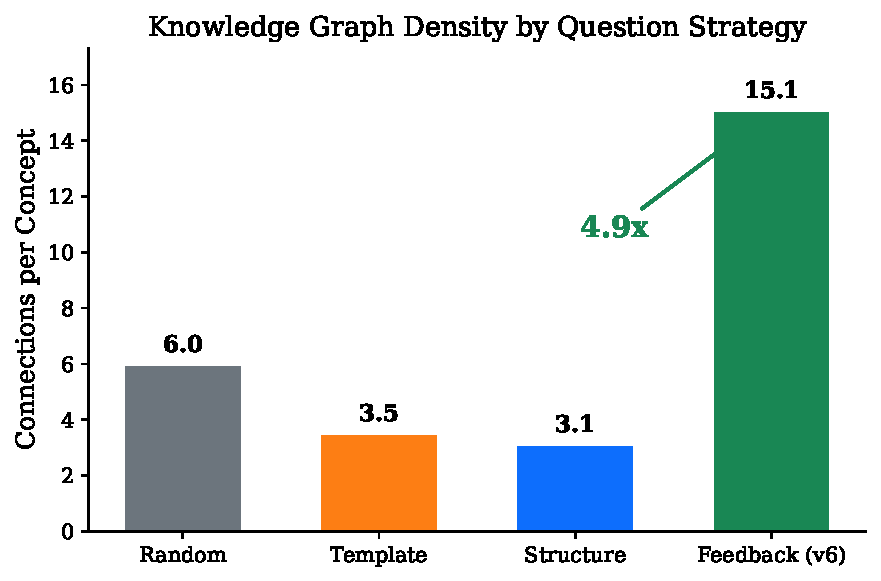
\includegraphics[width=0.85\textwidth]{figures/fig1_connections.pdf}
\caption{Connections per concept across four ablation modes. Feedback mode produces 4.9$\times$ more connections than structure without feedback.}
\label{fig:connections}
\end{figure}

\subsection{Cumulative Learning Rate}

Figure~\ref{fig:cumig} shows cumulative information gain over 200 steps. The feedback curve diverges from the others after approximately step 40, when the knowledge graph reaches sufficient density for structure-driven questions to become productive.

\begin{figure}[H]
\centering
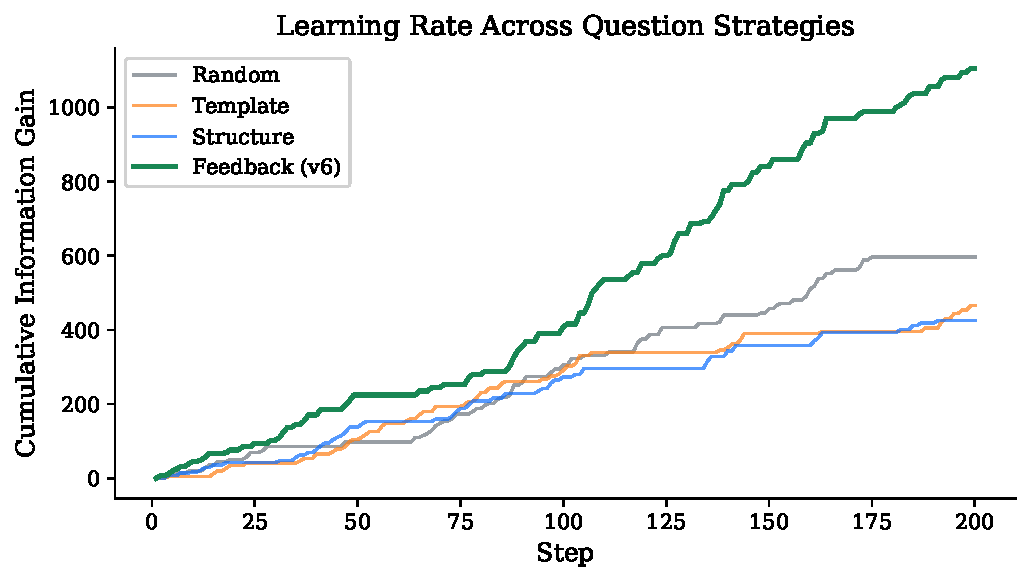
\includegraphics[width=0.85\textwidth]{figures/fig2_cumulative_ig.pdf}
\caption{Cumulative information gain over 200 steps. Feedback mode accelerates after step $\sim$40 as the knowledge graph becomes dense enough for structural questioning to outperform random exploration.}
\label{fig:cumig}
\end{figure}

\subsection{Strategy-Level Analysis}

\begin{figure}[H]
\centering
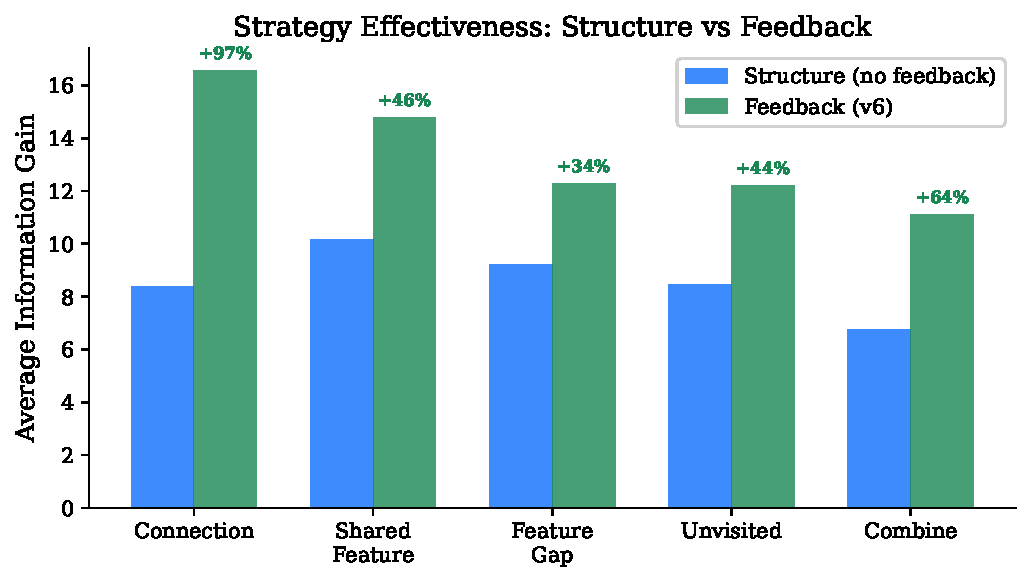
\includegraphics[width=0.85\textwidth]{figures/fig3_strategy_breakdown.pdf}
\caption{Average information gain per strategy: structure mode (equal weights) vs. feedback mode (learned weights). Every strategy improves with feedback.}
\label{fig:strategy}
\end{figure}

Critically, every strategy improves when feedback is enabled (Figure~\ref{fig:strategy}). The \texttt{connection} strategy shows the largest improvement (+97\%), followed by \texttt{combine} (+64\%), \texttt{shared\_feat} (+45\%), \texttt{unvisited} (+44\%), and \texttt{feature\_gap} (+34\%).

This is not simply a matter of selecting better strategies more often. The feedback loop creates a compounding advantage: better questions produce denser knowledge graphs, which give \emph{all} strategies richer material to work with. The improvement is systemic, not selective.

\subsection{Emergent Meta-Learning: Strategy Reversal}

The most striking result is a strategy reversal observed in the feedback run. At step 20, the \texttt{connection} strategy had the lowest average IG (2.4) of all strategies. By step 200, it had the highest (16.57). This reversal was not programmed---it emerged from the interaction between the feedback loop and the growing knowledge graph.

The explanation: \texttt{connection} questions require existing edges in the knowledge graph to be productive. At step 20, the graph has few connections, so connection-based questions produce little learning. But as the graph densifies (partly through other strategies), connection questions become increasingly productive because they leverage the accumulated structure.

\subsection{Why Structure Performs Worse Than Random}

Counterintuitively, structure-driven questioning without feedback (62 connections) performs worse than random exploration (119 connections). This is attributed to \emph{exploration rut}: without feedback, the structure mode defaults to a fixed distribution over strategies, with \texttt{feature\_gap} dominating (14 uses vs.\ 4 for \texttt{connection}). Feature-gap questions are the least connected to existing knowledge---they ask about what the graph \emph{lacks}---so they tend to produce isolated facts rather than bridging connections.

Random exploration, by contrast, occasionally stumbles into productive territory by accident. The absence of strategy imposes no constraint on exploration scope. This finding suggests that \textbf{informed exploration without adaptation is worse than uninformed exploration}, a result with implications for curriculum learning and active learning more broadly.

\subsection{Feedback Mode Asks More Questions}

Feedback mode produced 82 active steps compared to 48--58 for other modes. This is a secondary effect: higher-IG questions also produce more surprise in the embedding space, which triggers more active questioning cycles. Better questions do not just produce more learning per question---they also trigger \emph{more} questions. This positive feedback loop (better questions $\to$ more learning $\to$ more surprise $\to$ more questions) compounds the advantage of the feedback mode.


%% ============================================================
\section{Extended Run: 2000 Steps}
\label{sec:extended}

To test whether the feedback advantage persists at scale, an extended 2000-step run was conducted with the concept ceiling raised from 20 to 200. Key findings:

\begin{table}[H]
\centering
\begin{tabular}{lrrrr}
\toprule
\textbf{Scale} & \textbf{Concepts} & \textbf{Connections} & \textbf{Conn/Concept} & \textbf{Avg IG} \\
\midrule
200 steps (ceiling=20)  & 20  & 301    & 15.1  & 13.48 \\
2000 steps (ceiling=200) & 200 & 18,203 & 91.0  & 59.46 \\
\bottomrule
\end{tabular}
\caption{Feedback mode at two scales. Connection density scales superlinearly.}
\label{tab:extended}
\end{table}

\paragraph{Accelerating returns.} Information gain does not plateau---it accelerates. Average IG per 400-step window: 15.1 (steps 0--400), 38.3 (400--800), 61.7 (800--1200), 79.8 (1200--1600), 100.3 (1600--2000). This suggests the feedback loop compounds as the knowledge graph densifies, with each new connection creating opportunities for higher-value questions.

\paragraph{Question repetition.} Without question memory, the system repeated ``What is water?'' 14 times and ``What is bird?'' 8 times across 685 active steps. The structural seeds that generate questions are deterministic given the graph state: if the graph has not changed in the relevant neighbourhood since the last question, the same question is regenerated. This wastes approximately 3\% of active steps on exact duplicates and a larger fraction on near-duplicates. A self-referential extension that tracks question history is the primary target for the next version.

\paragraph{Concept quality.} Of the 200 concepts, 18 (9\%) are function words or morphological fragments (``ing'', ``don'', ``eted'') that passed the frequency-based growth filter. Semantic validation during neurogenesis would improve concept purity without requiring supervised filtering.


%% ============================================================
\section{Discussion}
\label{sec:discussion}

\subsection{The LLM as Environment}

The architectural choice to treat the LLM as an environment rather than a subject has several advantages:

\begin{enumerate}[leftmargin=*]
\item \textbf{Separation of concerns:} The outer layer decides \emph{what} to ask; the LLM decides \emph{how} to answer. Neither modifies the other's weights.
\item \textbf{Composability:} The same outer layer could interact with different LLMs, knowledge bases, or even human interlocutors.
\item \textbf{Interpretability:} The knowledge graph is an explicit, inspectable representation of what the system has learned.
\item \textbf{Bounded knowledge environments:} LLMs with limited training data (e.g., pre-1930 corpora) provide a natural ``knowledge wall'' for studying how an outer layer handles gaps and incoherence.
\end{enumerate}

\subsection{Limitations}

\begin{itemize}[leftmargin=*]
\item \textbf{No question memory:} The system maintains no record of past questions. At scale, this produces repetition: in a 2000-step extended run, ``What is water?'' was asked 14 times and ``What is bird?'' 8 times, because the same structural seeds regenerate the same questions. A self-referential system should know what it has already asked and why a question is worth re-asking. This is the most significant architectural gap.
\item \textbf{Concept quality at scale:} With the concept ceiling raised to 200, the system hit the ceiling in 2000 steps but 9\% of concepts (18/200) are function words (``ing'', ``don'', ``his'', ``she'') that leaked through the stopword filter. The feature-frequency growth mechanism needs semantic filtering, not just frequency thresholds.
\item \textbf{Ceiling effects:} Both the 200-step (ceiling=20) and 2000-step (ceiling=200) runs hit the concept ceiling. True concept discovery dynamics remain masked by the cap.
\item \textbf{Single seed:} All runs use seed 42. Results have not yet been verified as robust across seeds.
\item \textbf{Single model:} Llama 3 8B only. Different base models may produce different dynamics.
\item \textbf{No verification:} The system does not check whether the LLM's answers are correct. It trusts the environment. Incoherence detection is a necessary extension.
\end{itemize}

\subsection{The Recursive Insight}

There is a recursive quality to this research that bears noting. The system---which reflects on its accumulated knowledge graph to generate questions that produce new knowledge---mirrors the research process itself. The project began with a plan to study LoRA adapters, pivoted to surprise-driven exploration, then to concept learning, and finally to feedback-driven question generation. Each pivot was driven by reflecting on accumulated results and identifying the most productive next question. The outer layer's strategy reversal (from exploration to exploitation as structure accumulates) recapitulates the researcher's own trajectory.

This is not a claim about consciousness or understanding. It is an observation that the computational pattern---\emph{growing knowledge + structural reflection = emergent direction for new inquiry}---appears at multiple scales of the system.


%% ============================================================
\section{Related Work}
\label{sec:related}

\textbf{Curiosity-driven exploration} in reinforcement learning uses intrinsic motivation signals (prediction error, information gain, novelty) to guide agent behaviour \cite{pathak2017,burda2019}. The present approach differs in using a knowledge graph's structure rather than raw prediction error to define ``interesting'' directions.

\textbf{Active learning} selects training examples that maximise model improvement \cite{settles2009}. The system presented here extends this by generating queries rather than selecting from a pool.

\textbf{Knowledge graph construction} from text typically uses supervised information extraction \cite{ji2022}. The present system builds knowledge graphs through interaction rather than extraction, without labelled data or pre-defined relation types.

\textbf{LLM-based agents} that use language models as reasoning engines for task completion \cite{yao2023} share the framing of the LLM as a tool. However, these agents pursue externally defined goals; the present system pursues internally generated curiosity signals.


%% ============================================================
\section{Future Work}
\label{sec:future}

\paragraph{Bounded knowledge environments.} LLMs trained on restricted corpora (e.g., pre-1930 text) provide a controlled setting for studying how the outer layer handles knowledge boundaries. Preliminary manual experiments with such a model reveal three distinct failure modes---confabulation, domain substitution, and sense drift---that an outer layer must learn to detect.

\paragraph{Incoherence detection.} The current system trusts all LLM outputs. A production-grade system needs multi-signal verification: coherence checking against the knowledge graph, surprise detection, abstract rephrasing, and multi-probe convergence.

\paragraph{Self-synthesis.} When the base model cannot answer a question satisfactorily, the outer layer could attempt to synthesise an answer from its own knowledge graph---bridging concepts that the LLM never connected.


%% ============================================================
\section{Conclusion}
\label{sec:conclusion}

This paper presented a system where a lightweight outer layer autonomously builds knowledge by using a frozen LLM as an environment. The outer layer forms its own abstractions from accumulated experience and queries the LLM about these self-generated concepts, creating a cycle of abstraction and inquiry. A four-way ablation study demonstrates that how questions are generated matters enormously: feedback-driven strategy selection produces 4.9$\times$ denser knowledge graphs than structure-driven questioning without adaptation, and every individual strategy improves by 34--97\% when feedback is enabled.

The most striking finding is that informed exploration without adaptation performs \emph{worse} than random exploration. Structure alone constrains the exploration space too narrowly. Feedback is what transforms structure from a liability into an advantage.

The system exhibits emergent meta-learning: the worst strategy at step 20 becomes the best by step 200, driven entirely by the interaction between the feedback loop and the growing knowledge graph. This suggests that the relationship between knowledge structure and exploration strategy is dynamic and must be learned, not prescribed.


%% ============================================================
\section*{Reproducibility}

All code, data, and figures are available at:

\begin{center}
\url{https://github.com/aggarwalmew/dream-layer}
\end{center}

The ablation study can be reproduced with:

\begin{lstlisting}[language=bash,numbers=none]
python concept_learner.py --mode random    --steps 200 --seed 42 --reset
python concept_learner.py --mode template  --steps 200 --seed 42 --reset
python concept_learner.py --mode structure --steps 200 --seed 42 --reset
python concept_learner.py --mode feedback  --steps 200 --seed 42 --reset
\end{lstlisting}

Hardware: Apple M3 with 16GB RAM. Runtime: approximately 20 minutes per mode.


%% ============================================================
\begin{thebibliography}{9}

\bibitem{gopnik1999}
Gopnik, A., Meltzoff, A. N., and Kuhl, P. K.
\emph{The Scientist in the Crib: Minds, Brains, and How Children Learn}.
William Morrow, 1999.

\bibitem{pathak2017}
Pathak, D., Agrawal, P., Efros, A. A., and Darrell, T.
Curiosity-driven exploration by self-supervised prediction.
In \emph{ICML}, 2017.

\bibitem{burda2019}
Burda, Y., Edwards, H., Storkey, A., and Klimov, O.
Exploration by random network distillation.
In \emph{ICLR}, 2019.

\bibitem{settles2009}
Settles, B.
Active learning literature survey.
\emph{Computer Sciences Technical Report 1648}, University of Wisconsin--Madison, 2009.

\bibitem{ji2022}
Ji, S., Pan, S., Cambria, E., Marttinen, P., and Yu, P. S.
A survey on knowledge graphs: Representation, acquisition, and applications.
\emph{IEEE Transactions on Neural Networks and Learning Systems}, 33(2), 2022.

\bibitem{yao2023}
Yao, S., Zhao, J., Yu, D., et al.
ReAct: Synergizing reasoning and acting in language models.
In \emph{ICLR}, 2023.

\end{thebibliography}


\end{document}
